\chapter{Получение профильной информации из трасс исполнения}\label{ch:ch2}

В данной главе рассматривается разработанный универсальный метод получения профильной информации приложения из трасс исполнения.

В разделе 2.1 описывается метод получения трасс исполнения приложений на основе динамической бинарной инструментации и приводится предлагаемая схема оптимизации бинарного файла на ARM архитектуре.

В разделе 2.2 изложен алгоритм работы модели предсказателя переходов по трассе исполнения приложения, необходимый для получения информации о промахах предсказателя для профиля.

В разделе 2.3 приводится сравнение предлагаемого решения с уже существующим подходом работы бинарного оптимизатора BOLT. Сопоставляются профили, полученные на ARM и x86 архитектурах. Сравниваются подходы получения профильной информации с помощью аппаратной поддержки LBR и трасс исполнения приложения.

В разделе 2.4 описываются используемые синтетические тесты для проверки корректности работы предлагаемого метода получения профильной информации.

В разделе 2.5 приводятся результаты запусков оптимизированных на основе профильной информации, собранной из трасс исполнения, синтетических тестов.

\section{Получение трасс исполнения приложений}\label{sec:ch2/sec2}
Для анализа исполняемого файла без исходного кода применяется динамическая бинарная инструментация (DBI, Dynamic Binary Instrumentation). Во время работы приложения производится модификация программы с целью её анализа. С помощью инструментирующих процедур происходит вставка дополнительного кода \cite{Nethercote2007}. Это позволяет производить анализ во время возникновения в программе необходимых событий, таких как исключения, взятие переходов, создание процессов и т.д. \cite{Li2007}.

На основе данного подхода были реализованы DBI фреймворки, такие как Valgring \cite{Nethercote2003}, PIN, DynamoRIO \cite{Bruening2003} и DynInst \cite{Rimsa2019}. На их основе реализуются динамические бинарные анализаторы (DBA, Dynamic Binary Analysis), один из них был использован для сбора профильной информации для ARM архитектуры\cite{Hazelwood2006}. 

С помощью DBI фреймворка производится запись трассы исполнения приложения \cite{Hong2019}. Записывается последовательность инструкций, поступающих на процессор. После исполнения последовательность анализируется конвертером для генерации профиля исполнения, который записывается в формате BOLT (рисунок \cref{fig:NewSteps}). Такое решение приводит к замедлению работы оптимизируемого приложения в несколько раз, но создаёт трассу, которую можно анализировать без привязки к конкретной микроархитектуре. \cite{vakbib1} \cite{confbib2}

\begin{figure}[ht]
    \centerfloat{
        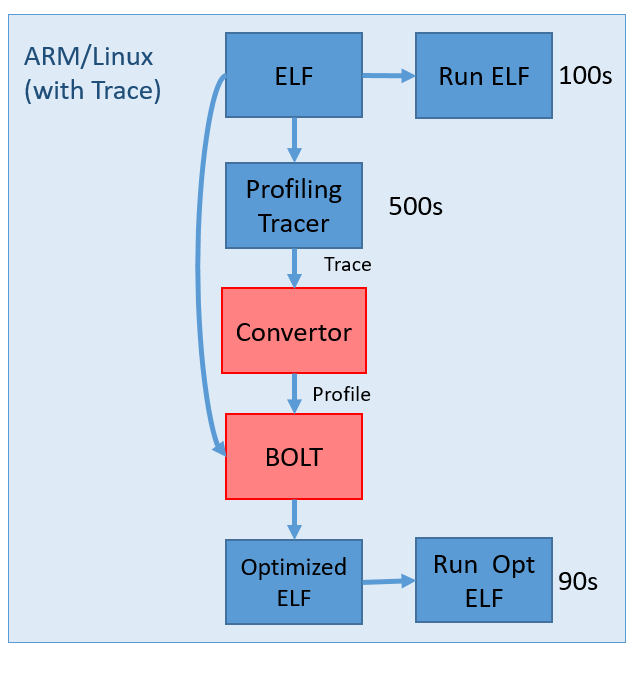
\includegraphics[width=0.6\linewidth]{9}
    }
    \caption{Предлагаемая схема оптимизации бинарного файла на ARM архитектуре}\label{fig:NewSteps}
\end{figure}

\section{Моделирование предсказателя переходов}\label{sec:ch2/sec3}
Чтобы получить информацию о переходах для профиля, конвертер проходит по всей трассе и находит инструкции меняющие поток управления: B, BR, BL, BLR, B.cond, TBZ, TBNZ, CBZ, CBNZ, RET (рисунок \cref{fig:ProfilefromTrace}) \cite{Kalla2017}. После чего информация поступает в модель предсказателя переходов (Branch Predictor Model). Данная модель выбирается в зависимости от конкретной микроархитектуры процессора, для которого оптимизируется приложение. В итоге собирается информация для получения количества не предсказанных и количества взятых переходов \cite{Ball1993} \cite{Fisher1992}.

\begin{figure}[ht]
    \centerfloat{
        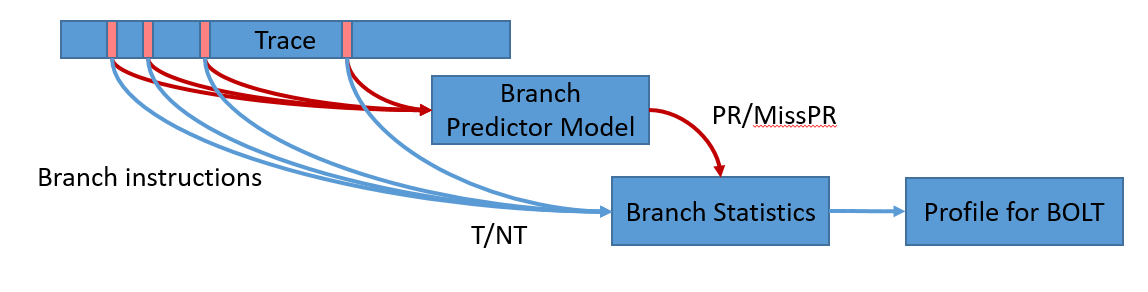
\includegraphics[width=1.0\linewidth]{10}
    }
    \caption{Схема генерации профиля из трассы исполнения}\label{fig:ProfilefromTrace}
\end{figure}

Для используемых в рамках данной работы устройств была реализована модель обрабатывающая три типа событий:
\begin{enumerate}[beginpenalty=10000]
  \item Безусловный переход по адресу.
  \item Условный переход по адресу.
  \item Косвенный переход по регистру.
\end{enumerate}

Безусловный переход по адресу обрабатывается без работы модели. Событие перехода сразу попадает в статистику переходов программы со значением предсказания 100\%.

Во втором случае необходимо получить данные из модели предсказателя перехода о том, был ли сделан переход, или исполнение пошло на следующую инструкцию, то есть условие перехода было на выполнено. После чего производится сравнение с реальным ходом исполнения трассы и проверяется, было ли верно сделано предсказание. Этот результат записывается в статистику переходов.

Для обработки данных вариантов была реализована модель, наиболее близкая к заявленной на ARM Cortex A76: гибридная модель, сочетающая в себе бимодальный и глобальный предсказатели. Глобальный предсказатель использовался с 16--битной историей, а для вычисления индекса производилась операция исключающее <<ИЛИ>> с 6 битами адреса текущего перехода \cite{Smith1981}.

В случае события косвенного перехода по регистру с помощью предсказателя целевого адреса вычисляется возможный переход, который сверяется по трассе с реально сделанным. Для этой задачи используется буфер целевых адресов (BTB, Branch Target Buffer) размером 8 со случайным замещением записей \cite{Ajorpaz2018}.

В итоге процессирования всей трассы и работы моделей получается результирующая статистика со значениями количества сделанных и предсказанных переходов, из которой генерируется профиль в формате BOLT.

Также стоит отметить, что описанный подход позволяет процессировать несколько трасс подряд, позволяя объединять информацию о нескольких запусках и более полно покрывать оптимизируемое приложение.

\section{Проверка профильной информации, полученной с трасс исполнения}\label{sec:ch2/sec4}
В сравнении с оригинальным методом сбора профиля на основе LBR данный подход имеет ряд преимуществ. Во-первых, трасса исполнения зависит только от архитектуры, но не микроахитетктуры устройства, на котором происходит динамическая бинарная инструментация, что означает возможность повторной оптимизации приложения под другую микроархитектуру с другой моделью предсказателя переходов. Во-вторых, собранный профиль покрывает всё исполнение оптимизируемого приложения, а не часть исполнения как в случае с LBR. Таким образом, полученная информация более корректна, так как избавляет профиль от искажений, связанных с ожиданием готовности периферии процессора, например, обращение в память.
На рисунке \cref{fig:LBRvsTRace} продемонстрирована разница между сбором информации с помощью LBR и трассы исполнения. В данном примере берётся упрощенная модель LBR с 4 записями о последней инструкции, которые будут попадать в профиль при срабатывании события записи. Конвертер при анализе будет учитывать каждую инструкцию перехода.

 
\begin{figure}[ht]
    \centerfloat{
        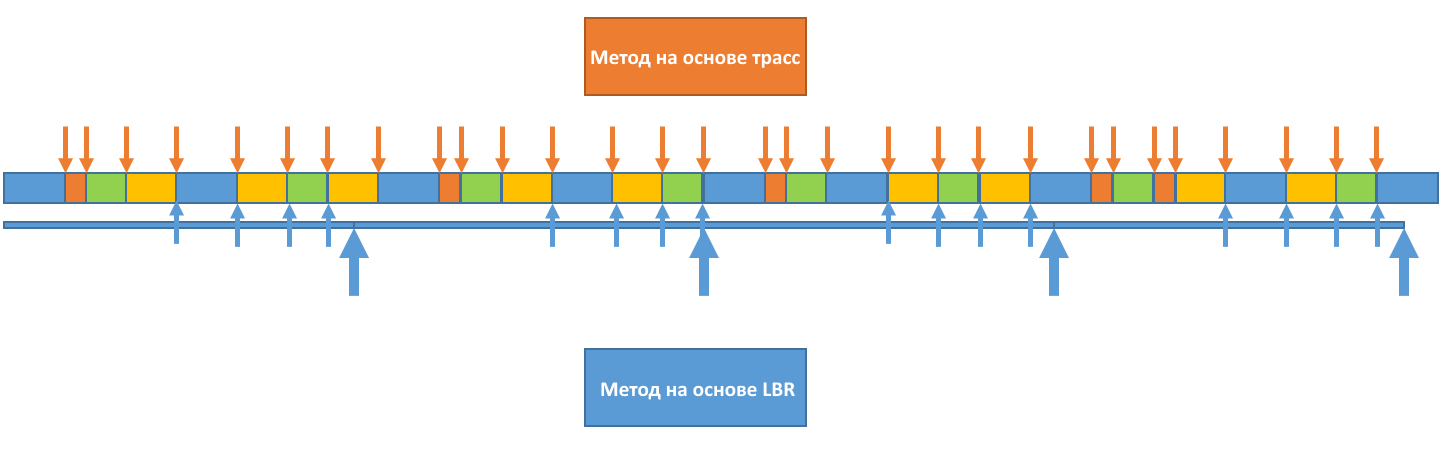
\includegraphics[width=1.0\linewidth]{vs1}
    }
    \caption{Сравнение методов сбора профильной информации}\label{fig:LBRvsTRace}
\end{figure}

Разные методы сбора профильной информации приводят к генерации различных профилей. В данном примере LBR не будет учитывать горячий переход между синим и красным базовыми блоками, что приведёт к не оптимальным преобразованиям бинарного файла (рисунок \cref{fig:LBRvsTraceRes}).
 
\begin{figure}[ht]
    \centerfloat{
        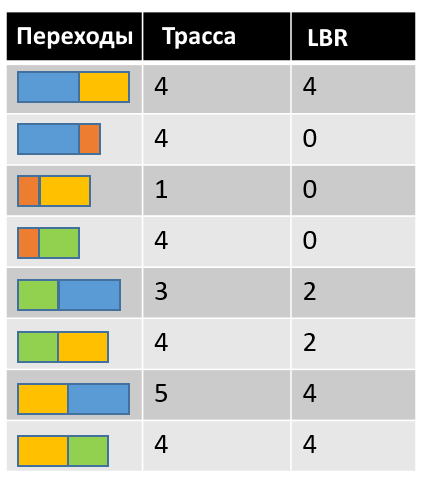
\includegraphics[width=0.5\linewidth]{vs2}
    }
    \caption{Профили, полученные с помощью трассы и LBR}\label{fig:LBRvsTraceRes}
\end{figure}

	Если рассматривать данный пример при большем времени исполнения, то статистически профили будут получены одинаковые. При этом если добавить задержку на обращение в память, то более горячими базовыми блоками станут те, на которых происходило ожидание чтение/записи данных и N-1 предыдущих базовых блоков, где N – размер буфера LBR. Так как основная цель данной оптимизации является улучшение работы инструкционного кэша, то возникает искажение профиля, приводящая к понижению средней температуры L1i.

Метод сбора профильной информации с использованием трассы исполнения был проверен на приложениях, собранных под архитектуру ARM. Для аналогичных программ под x86 собранные с помощью LBR профили коррелируют с полученными выше, что позволяет использовать динамическую бинарную инструментацию с последующим анализом переходов для использования с BOLT.

Профиль, сгенерированный с помощью трасс, для демонстрационного примера изображен в таблице \cref{tab:ARMTrace}.
\begin{table} [h]% Пример записи таблицы с номером, но без отображаемого наименования
    \centering
    \begin{threeparttable}% выравнивание подписи по границам таблицы
        \caption{Профиль демонстрационного примера на ARM архитектуре, собранный с трассы исполнения приложения}%
        \label{tab:ARMTrace}%
        \begin{SingleSpace}
            \begin{tabular}{| c | c | c | c | c | c | c | c |}
                \hline
				1& main& 150& 0& [unknown]& 0& 1& 1 \\ \hline
				0& [unknown]& 0& 1& main& 13c& 1& 1 \\ \hline
				1& falseFunc& 6c& 1& main& 104& 6309097& 6309097 \\ \hline
				1& falseFunc& 60& 1& falseFunc& 28& 0& 28391358 \\ \hline
				1& falseFunc& 34& 1& falseFunc& 64& 6256725& 6309097 \\ \hline
				1& falseFunc& 34& 1& falseFunc& 38& 0& 28391358 \\ \hline
				1& falseFunc& 24& 1& falseFunc& 28& 0& 6309097 \\ \hline
				1& main& 100& 1& falseFunc& 0& 0& 6309097 \\ \hline
				1& main& 120& 1& main& 68& 0& 9999999 \\ \hline
				1& main& dc& 1& main& 110& 0& 3690902 \\ \hline
				1& trueFunc& 6c& 1& main& d0& 3690902& 3690902 \\ \hline
				1& main& cc& 1& trueFunc& 0& 0& 3690902 \\ \hline
				1& condition& 78& 1& main& a8& 9999999& 9999999 \\ \hline
				1& main& a4& 1& condition& 0& 0& 9999999 \\ \hline
				0& [unknown]& 0& 1& main& 94& 9999999& 9999999 \\ \hline
				1& main& 78& 1& main& 124& 75& 1 \\ \hline
				1& main& 78& 1& main& 7c& 0& 9999999 \\ \hline
				1& main& 64& 1& main& 68& 0& 1 \\ \hline
				0& [unknown]& 0& 1& main& 0& 1& 1 \\ \hline
				1& trueFunc& 60& 1& trueFunc& 28& 0& 16608642 \\ \hline
				1& trueFunc& 34& 1& trueFunc& 64& 4429145& 3690902 \\ \hline
				1& trueFunc& 34& 1& trueFunc& 38& 0& 16608642 \\ \hline
				1& trueFunc& 24& 1& trueFunc& 28& 0& 3690902 \\ \hline
				1& \_start& 4& 1& do\_arm64\_start/1& 0& 0& 1 \\ \hline
				0& [unknown]& 0& 1& \_start& 0& 1& 1 \\ \hline
				1& main& a8& 1& main& e0& 2347424& 6309097 \\ \hline
				1& main& a8& 1& main& ac& 0& 3690902 \\ \hline
				0& [unknown]& 0& 1& condition& 3c& 9999999& 9999999 \\ \hline
				1& main& 110& 1& main& 114& 0& 9999999 \\ \hline
				1& main& 10c& 1& main& 110& 0& 6309097 \\ \hline
				1& main& 20& 1& main& 54& 0& 1 \\ \hline
            \end{tabular}%
        \end{SingleSpace}
    \end{threeparttable}
\end{table}
	
Точное сравнение профилей невозможно сделать по двум причинам:
\begin{enumerate}[beginpenalty=10000]
  \item Различие в архитектурах и самих бинарных файлов.
  \item Различие методов сбора профильной информации приложения.
\end{enumerate}

Поэтому сравнение производилось по соотношению основных показателей статистики по тем переходам, по которым можно построить соответствие с исходным кодом. Например, 12 строчка демонстрационного кода (рисунок \cref{fig:TestCode}) соответствует инструкции CBZ по адресу 0x98C (Приложение \cref{lst:ARM}, Листинг Б.1) в бинарном файле для ARM архитектуры и инструкции JE по адресу 0x135E (Приложение \cref{lst:X86}, Листинг Б.2) в бинарном файле для x86 архитектуры.

Полученные адреса инструкций необходимо найти в соответствующей профильной информации. Для ARM архитектуры из таблицы \cref{tab:ARMTrace} следует запись \textbf{1 main a8 1 main e0 2347424 6309097} (так как адрес начала функции main 0x8E4), а для x86 архитектуры запись из таблицы \cref{tab:X86LBR} \textbf{1 main 9e 1 main cd 317 730} (так как адрес начала функции main 0x12C0).

Также в профильной информации есть особенность записи для условных переходов. Для каждой такой инструкции будет сгенерировано две записи:
\begin{enumerate}[beginpenalty=10000]
  \item Запись из инструкции перехода в целевой адрес с указанием предсказанных и взятых исполнений.
  \item Запись из инструкции перехода на следующую инструкцию (при не выполнении условия). При этом в информации от предсказателя переходов нет необходимости.
\end{enumerate}

Для выбранного перехода второй тип записи будет следующим: \textbf{1 main a8 1 main ac 0 3690902} для примера на ARM (таблица \cref{tab:ARMTrace}) и \textbf{1 main 9e 1 main a4 0 421} для x86 (таблица \cref{tab:X86LBR}).

Чтобы проверить корректность полученного профиля для ARM, необходимо сравнить соотношение взятых переходов первого типа записи ко второму. Для обеих архитектур оно должно получиться одинаковым в том случае, если функция condition работает идентично на всех случаях. Полученные значения: 0.58 для ARM и 0.57 для x86 показывают корректность полученного профиля.

\begin{figure}[!h]
    \centerfloat{
        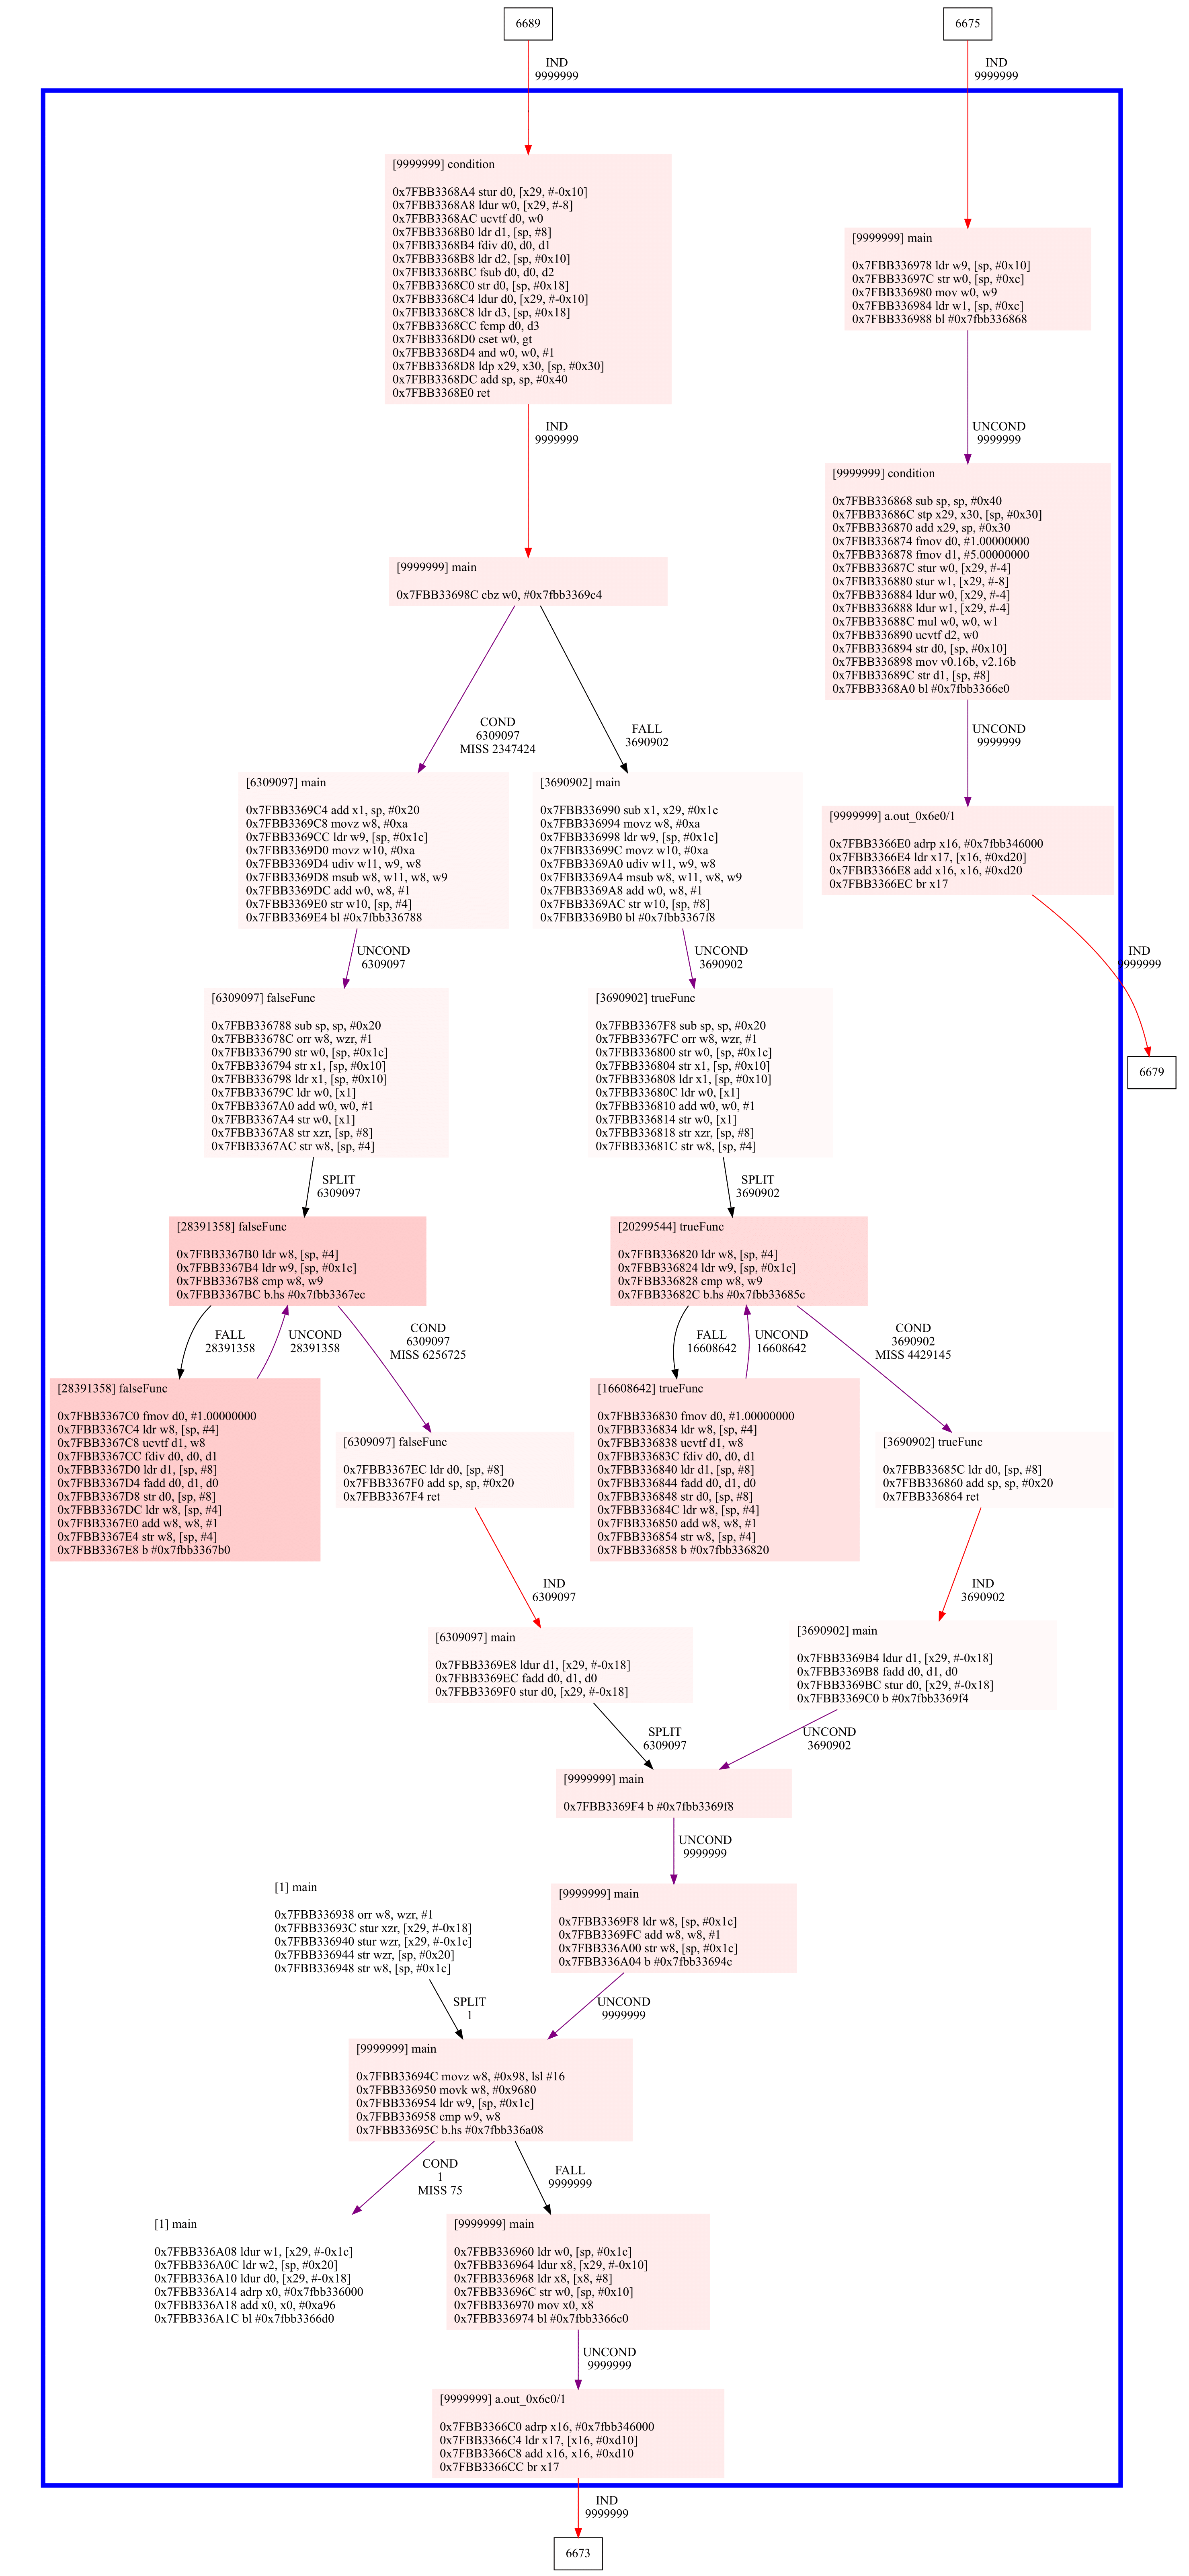
\includegraphics[width=0.6\linewidth]{ARM_graph-1}
    }
    \caption{Граф управления синтетического теста с профильной информацией}\label{fig:DEMOCFG}
\end{figure}

По синтетическому примеру с записанной трассы был собран граф потока управления (рисунок \cref{fig:DEMOCFG}), позволяющий проанализировать работу приложения и часто исполняемые участки кода (более красные линейные участки - чаще исполняемые).

\section{Описание синтетических тестов}\label{sec:ch2/sec5}
Для проверки прироста производительности предложенного метода  сбора профильной информации искусственно были созданы тесты, в которых исполняемый код перемешан с неисполняемым холодным кодом, что приводит к неэффективному использованию инструкционного кэша. Для генерации бинарного файла большого размера (> 10 МБ) применяется рекурсивный вызов шаблонных функций в языке программирования C++. С их помощью компилятор создавал множественные копии функций с разными шаблонными константами, тем самым увеличивая размер кода до нужного значения. Исполняемый код равномерно распределяется по секции, перемежаясь с холодными функциями. 
Примеры синтетических тестов приведены в Приложении \cref{app:A}.

Изначально был сделан тест без стандартной библиотеки для того, чтобы потенциально сложных для бинарного оптимизатора мест было как можно меньше (Приложение \cref{app:A}, Листинг A.1).

В тестовом примере в цикле hot\_repeat раз  производятся рекурсивные вычисления с помощью функций hotFunc<CODE\_SIZE>. Шаблонный параметр выбирается таким, чтобы компилятор сгенерировал бинарный файл большого размера, так как будут созданы экземпляры для всех функций, используемых в программе, с параметрами от CODE\_SIZE до 0 с шагом 1.

\begin{ListingEnv}[h]
    \captiondelim{ } % разделитель идентификатора с номером от наименования
    \caption{Функция main синтетического примера без стандартной библиотеки}\label{lst:hwplain}
    \begin{lstlisting}[language={[ISO]C++}]
    calcFunc<CODE_SIZE>(1);
    for (unsigned int i = 0; i < hot_repeat; i++)
    {
        hotFunc<CODE_SIZE>(1);
    }
    return 0;
    \end{lstlisting}
\end{ListingEnv}%

Для того чтобы генерация всех шаблонов прошла успешно, перед циклом вызывается функция calcFunc<CODE\_SIZE>, заставляющая компилятор создать все экземпляры. Эта функция отвечает за вычисления значений и несёт в себе вычислительную нагрузку данного теста. Она является аналогом демонстрационного приложения с рисунка \cref{fig:TestCode}.

\begin{ListingEnv}[!h]
    \captiondelim{ }
    \caption{Функция calcFunc синтетического примера без стандартной библиотеки}\label{lst:hwbeauty}
    \begin{lstlisting}[language={[ISO]C++}]
template<unsigned int param>
double calcFunc(unsigned int calc_args) 
{
    double res = 0.0;
    unsigned int TRUE = 0, FALSE = 0;
    unsigned int arg = param % 3;
    unsigned int itNumber = calc_args;
    
    if (itNumber == UINT_MAX) {
        calcFunc<param-1>(calc_args);
    }

    for (unsigned int i = 1; i <= itNumber; i++)
    {
        if (condition<param>(i, arg))
        {
            res += trueFunc<param>(i, &TRUE);
        } else {
            res += falseFunc<param>(i, &FALSE);
        }
    }
    return res;
}
    \end{lstlisting}
\end{ListingEnv}%

В теле функции есть вызов самой себя, но с декрементированным шаблонным параметром. Это создаст рекурсивный вызов шаблонных функций до нулевого параметра, так как в коде прописана специализация случая calcFunc<0>. При этом условие написано так, что на входных значения оно выполняться не будет, но код компилятор должен сгенерировать.

После того как один раз были созданы все экземпляры функций calcFunc, condition, trueFunc и falseFunc, размер бинарного файла стал нужного размера. В цикле функции main будет исполняться hotFunc, которая рекурсивно вызывает себя с шагом шаблонного параметра CODE\_STEP. Данный подход помогает чередовать часто используемые функции с не используемыми в бинарном файле.

\begin{ListingEnv}[!h]
    \captiondelim{ }
    \caption{Функция hotFunc синтетического примера без стандартной библиотеки}\label{lst:hwbeauty}
    \begin{lstlisting}[language={[ISO]C++}]
template<unsigned int param>
double hotFunc(unsigned int calc_args)
{
    return calcFunc<param>(calc_args) + hotFunc<param - CODE_STEP>(calc_args);
}
    \end{lstlisting}
\end{ListingEnv}%

Для компиляции примера без использования стандартной библиотеки необходимо написать стартовый файл на ассемблере целевой архитектуры. Примеры стартовых файлов приведены в Приложении \cref{app:A}, Листинг A.2 для ARM архитектуры и Листинг A.3 для архитектуры x86.

Второй тест написан уже с использованием стандартной библиотеки, что позволяет использовать вывод в консоль и проверить корректность вычисляемых значений (Приложение \cref{app:A}, Листинг A.4).

Последний тест написан с дополнением в виде использования исключений и виртуальных функций для проверки работы бинарного оптимизатора BOLT на подобных примерах (Приложение \cref{app:A}, Листинг A.5).

\section{Результаты тестирования}\label{sec:ch2/sec6}
Полученные статистические данные (рисунок \cref{fig:SynRes}) показывают понижение практически до нуля количество промахов по iTLB, увеличение IPC (instruction per clock) на 41\% и уменьшение времени работы на 29\%. Как было сказано выше, для тестирования была выбрана микроархитектура ARM Cortex A76 \cite{vakbib1}.
\begin{figure}[!h]
    \centerfloat{
        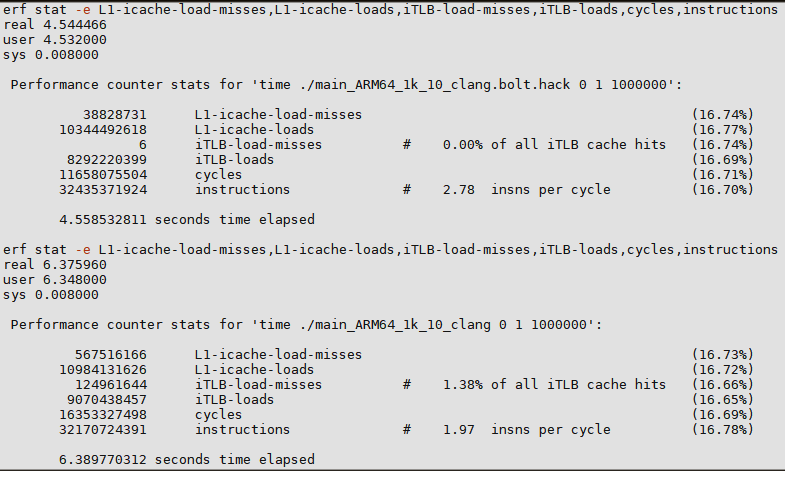
\includegraphics[width=1.0\linewidth]{13}
    }
    \caption{Сравнение результатов запусков оригинального и оптимизированного бинарных файлов синтетического теста}\label{fig:SynRes}
\end{figure}

Данные результаты повторяются на всех синтетических тестах, включая три теста, описанных в предыдущем разделе. На всех оптимизированных тестах отсутствуют промахи по iTLB в случае, когда суммарный размер часто исполняемых линейных участков не превышает размера отображаемого кода iTLB.

\section{Вывод по главе}\label{sec:ch2/sec7}
Во второй главе проводится анализ существующего подхода в бинарном оптимизаторе BOLT, который позволил предложить альтернативный способ получения профильной информации приложения на основе трасс исполнения.

Предлагаемая схема оптимизации бинарного файла на ARM архитектуре была протестирована на синтетических тестах.
\newpage
Также было проведено сравнение подходов на основе аппаратной поддержки с LBR и на основе трасс исполнения. Анализ полученных профилей подтверждает корректность применения предложенного подхода.

Приводимые результаты запусков, которые были оптимизированы на основе профильной информации, собранной из трасс исполнения синтетических тестов, подтверждают возможность использования данного метода.

\clearpage